\documentclass[12pt]{article}
\usepackage{amsmath, hyperref, multicol, fullpage}

\usepackage[usenames,dvipsnames]{xcolor} % allows you to use color names, call this BEFORE you call TikZ

\usepackage{tikz, tikz-3dplot, pgfplots}
\usepackage{tkz-graph}
\usetikzlibrary[positioning,patterns] % tikz libraries for relative positioning and silly patterns

% let pgfplots know what version you're using
\pgfplotsset{compat=1.8}

% Tyson's macros for Young tableau squares and big dominoes
\tikzstyle{bsq}=[rectangle, draw, thick, minimum width=1cm, minimum height=1cm] 
\tikzstyle{bver}=[rectangle, draw, thick, minimum width=1cm, minimum height=2cm]
\tikzstyle{bhor}=[rectangle, draw, thick, minimum width=2cm, minimum height=1cm]

% formatting the section titles
\usepackage{titlesec}
\titleformat{\section}{\large\bfseries}{\thesection}{1em}{}

% macro for TikZ logo
\newcommand{\TikZ}{Ti$k$Z }

\title{\TikZ/PGF and other \LaTeX  \, Tricks}    
\author{Erica Shannon}
\date{}

\begin{document}

\setlength\parindent{0pt}

\maketitle

\tableofcontents

\vfill

\TikZ stands for \TikZ ist \emph{kein} Zeichenprogramm; PGF stands for Portable Graphics Format.

\vfill

\section{Resources}

\footnotesize

\begin{itemize}
\item Comprehensive \TikZ Manual: \\ \url{http://ftp.math.purdue.edu/mirrors/ctan.org/graphics/pgf/base/doc/generic/pgf/pgfmanual.pdf}
\item \ttfamily pgfplots \rmfamily Manual: \\ \url{http://www.bakoma-tex.com/doc/latex/pgfplots/pgfplots.pdf}
\item A nice tutorial for basic drawing using \TikZ: \\ \url{http://www.math.uni-leipzig.de/~hellmund/LaTeX/pgf-tut.pdf}
\item List of colors available from the \ttfamily dvipsnames \rmfamily package: \\ \url{http://en.wikibooks.org/wiki/LaTeX/Colors}
\end{itemize}

\normalsize

\newpage
\section{Polygons}

Here are some triangles with labels.

\bigskip

\begin{center} 
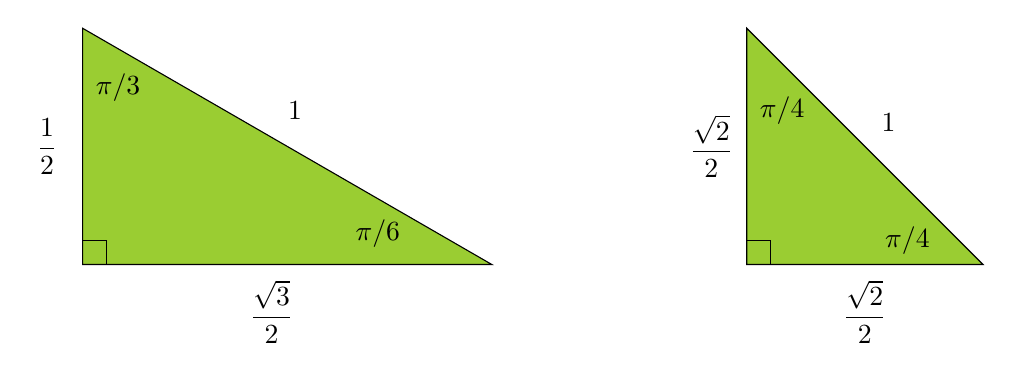
\begin{tikzpicture}[scale=3]
	
	\draw[fill=YellowGreen] (0,0) -- (1.732050808,0) -- (0,1) -- cycle;
	\draw (0,.1) -- (.1,.1) -- (.1,0);
	
	\node at (.15,.75) {$\pi / 3$};
	\node at (1.25,.13) {$\pi/6$};
	
	\node at (.9,.65) {1};
	\node at (-.15,.5) {$\displaystyle \frac{1}{2}$};
	\node at (.8, -.2) {$\displaystyle \frac{\sqrt{3}}{2}$};

\begin{scope}[xshift=80] % shifts everything enclosed in this to the right
	
	\draw[fill=YellowGreen] (0,0) -- (1,0) -- (0,1) -- cycle;
	\draw (0,.1) -- (.1,.1) -- (.1,0);
	
	\node at (.15,.65) {$\pi / 4$};
	\node at (.68,.1) {$\pi/4$};
	
	\node at (.6,.6) {1};
	\node at (-.15,.5) {$\displaystyle \frac{\sqrt{2}}{2}$};
	\node at (.5, -.2) {$\displaystyle \frac{\sqrt{2}}{2}$};
\end{scope}

\end{tikzpicture}
\end{center}   

\bigskip


Here are some regular polygons, drawn using the \ttfamily foreach \rmfamily command for~loops.

\bigskip

\begin{center}
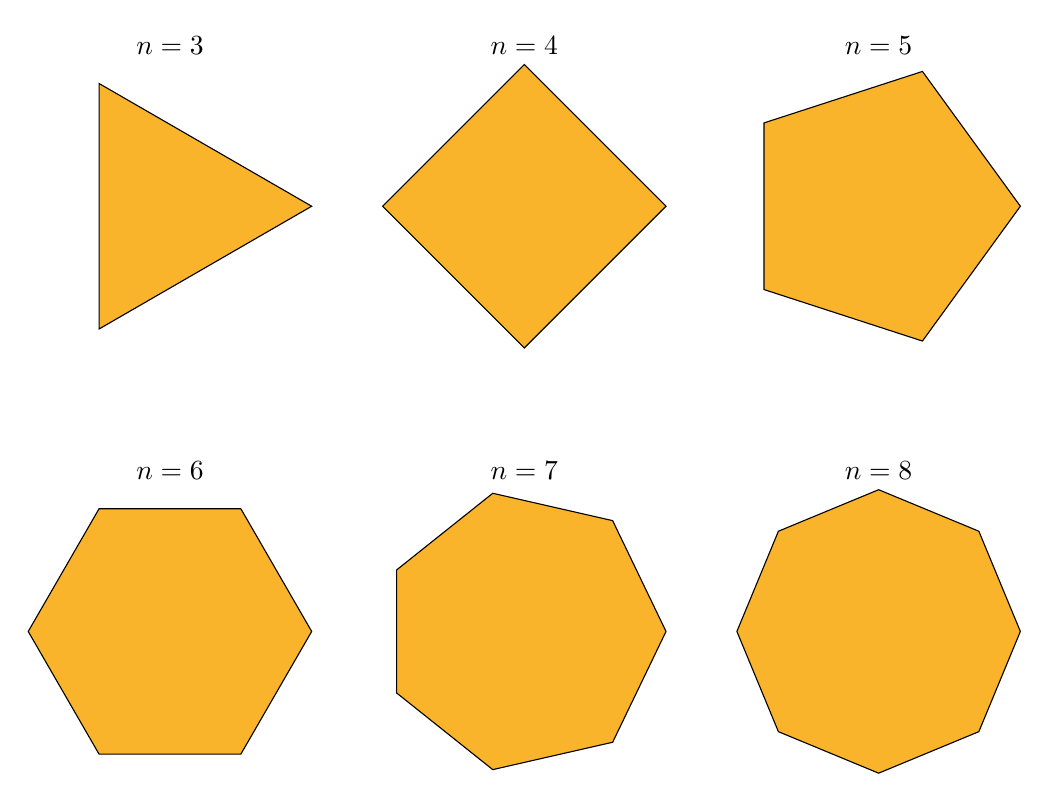
\begin{tikzpicture}

	\newdimen\R
	\R=1.8cm % this means each polygon will be inscribed in a circle of radius 1.8 cm.
	
	% all coordinates given below are polar coordinates in the form (angle : radius)
	
	\draw[fill=Dandelion] (0:\R) \foreach \x in {120,240} { -- (\x:\R) } -- cycle (90:\R) node[above] {$n=3$} ; 
	
	\draw[fill=Dandelion,xshift=2.5\R] (0:\R) \foreach \x in {90,180,...,359} {--(\x:\R)}--cycle (90:\R) node[above] {$n=4$} ;
	
	\draw[fill=Dandelion,xshift=5.0\R] (0:\R) \foreach \x in {72,144,...,359} {--(\x:\R)}--cycle (90:\R) node[above] {$n=5$} ;
	    
	\draw[fill=Dandelion,yshift=-3\R] (0:\R) \foreach \x in {60,120,...,359} {-- (\x:\R)}--cycle (90:\R) node[above] {$n=6$} ;
	                    
	\draw[fill=Dandelion, yshift=-3\R,xshift=2.5\R] (0:\R) \foreach \x in {51.4286,102.8571,...,359} {-- (\x:\R)}--cycle (90:\R) node[above] {$n=7$} ;
	
	\draw[fill=Dandelion,yshift=-3\R,xshift=5.0\R] (0:\R) \foreach \x in {45,90,...,359} {-- (\x:\R)} -- cycle (90:\R) node[above] {$n=8$} ;

\end{tikzpicture}
\end{center}

\bigskip 

The TikZ manual has examples of how to draw pretty much any type of shape or diagram you might come up with. In particular, there's a list of cool available node shapes starting on p.435. (Forbidden sign, clouds, magnifying glass, starburst, etc.)

\newpage
\section{Subgroup Lattices}

There is supposed to be a \TikZ library (\ttfamily graphs\rmfamily) for typesetting graphs. However, I found it extremely difficult to get this library to work correctly (or at all!). As a result, the examples here are made using the standard \TikZ nodes and lines.

\begin{center}
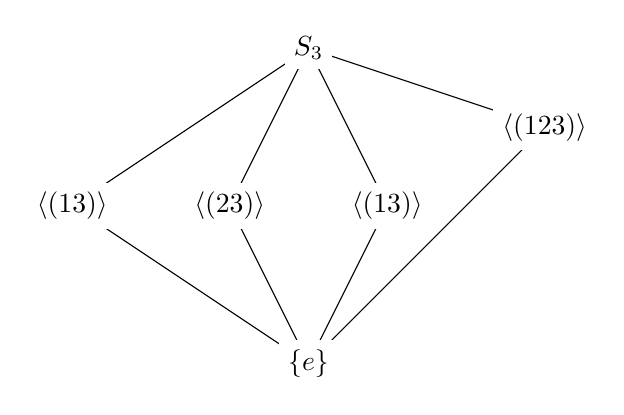
\begin{tikzpicture}[every node/.style={fill=white}] % white fill keeps lines from running into labels

	\draw (0,6) -- (3,5) -- (0,2);	
	\draw (0,6) -- (1,4) -- (0,2);
	\draw (0,6) -- (-1,4) -- (0,2);
	\draw (0,6) -- (-3,4) -- (0,2);

	\node at (0,6) {$S_3$};
	\node at (3,5) {$\langle (123) \rangle$};
	\node at (1,4) {$\langle(13)\rangle$};
	\node at (-1,4) {$\langle(23)\rangle$};
	\node at (-3,4) {$\langle(13)\rangle$};
	\node at (0,2) {$\{e\}$};

\end{tikzpicture}
\end{center}

Here's a more complicated one:

\begin{center}
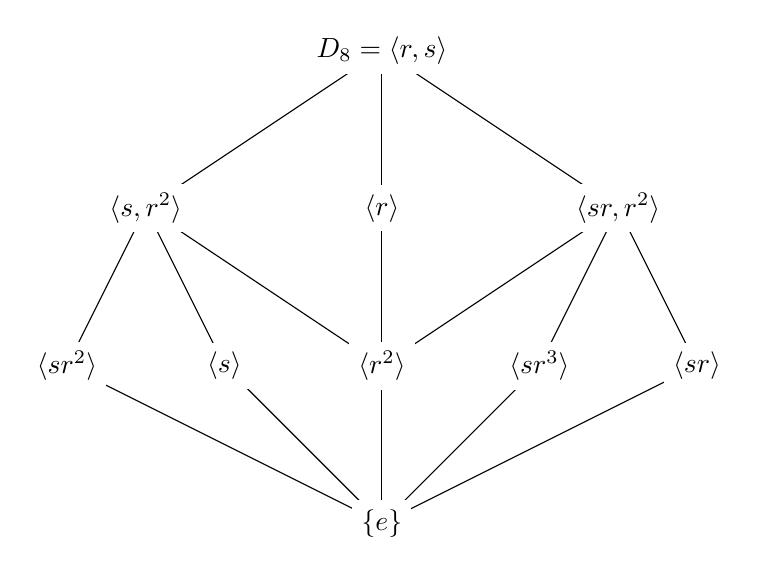
\begin{tikzpicture}[every node/.style={fill=white}]

	\draw (0,8) -- (0,2);	
	\draw (0,8) -- (3,6) -- (0,4);
	\draw (0,8) -- (-3,6) -- (0,4);
	\draw (3,6) -- (2,4) -- (0,2);
	\draw (-3,6) -- (-2,4) -- (0,2);
	\draw (3,6) -- (4,4) -- (0,2);
	\draw (-3,6) -- (-4,4) -- (0,2);

	\node at (0,8) {$D_8 = \langle r,s\rangle$};
	\node at (0,6) {$\langle r \rangle$};
	\node at (0,4) {$\langle r^2 \rangle$};
	\node at (0,2) {$\{e\}$};

	\node at (-3,6) {$\langle s, r^2 \rangle$};
	\node at (3,6) {$\langle sr, r^2 \rangle$};
	
	\node at (-4,4) {$\langle s r^2 \rangle$};
	\node at (-2,4) {$\langle s \rangle$};
	\node at (2,4) {$\langle s r^3 \rangle$};
	\node at (4,4) {$\langle sr \rangle$};

\end{tikzpicture}
\end{center}

\newpage
\section{Coxeter graphs and Dynkin diagrams}

Finite Coxeter groups can be classified by their Coxeter graphs.

\begin{multicols}{2}

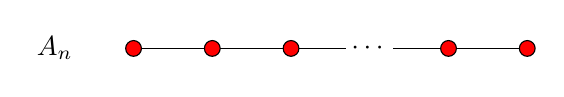
\begin{tikzpicture}
	
	\draw (0,0) -- (2.7,0);
	\draw (3.3, 0) -- (5,0);
	
	\draw[fill=red] (0,0) circle (.1);
	\draw[fill=red] (1,0) circle (.1);
	\draw[fill=red] (2,0) circle (.1);
	\draw[fill=red] (4,0) circle (.1);
	\draw[fill=red] (5,0) circle (.1);
	
	\node at (3,0) {$\cdots$};
	\node at (-1,0) {$A_n$};
	 
\end{tikzpicture}

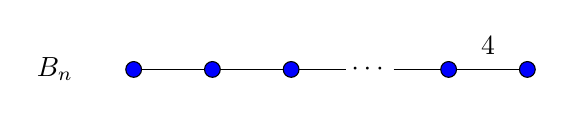
\begin{tikzpicture}

	\draw (0,0) -- (2.7,0);
	\draw (3.3, 0) -- (5,0);
	
	\draw[fill=blue] (0,0) circle(.1);
	\draw[fill=blue] (1,0) circle(.1);
	\draw[fill=blue] (2,0) circle(.1);
	\draw[fill=blue] (4,0) circle(.1);
	\draw[fill=blue] (5,0) circle(.1);
	
	\node at (3,0) {$\cdots$};
	\node at (4.5,.3) {4};
	\node at (-1,0) {$B_n$};
	 
\end{tikzpicture}

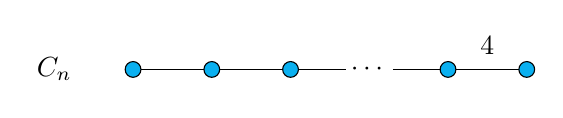
\begin{tikzpicture}

	\draw (0,0) -- (2.7,0);
	\draw (3.3, 0) -- (5,0);
	
	\draw[fill=ProcessBlue] (0,0) circle(.1);
	\draw[fill=ProcessBlue] (1,0) circle(.1);
	\draw[fill=ProcessBlue] (2,0) circle(.1);
	\draw[fill=ProcessBlue] (4,0) circle(.1);
	\draw[fill=ProcessBlue] (5,0) circle(.1);
	
	\node at (3,0) {$\cdots$};
	\node at (4.5,.3) {4};
	\node at (-1,0) {$C_n$};
	 
\end{tikzpicture}

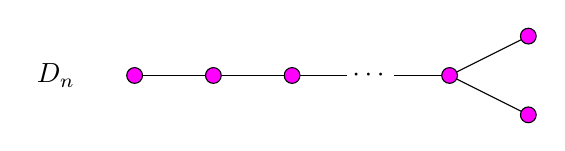
\begin{tikzpicture}

	\draw (0,0) -- (2.7,0);
	\draw (3.3, 0) -- (4,0);
	\draw (4,0) -- (5,-.5);
	\draw (4,0) -- (5,.5);
	
	\draw[fill=Magenta] (0,0) circle(.1);
	\draw[fill=Magenta] (1,0) circle(.1);
	\draw[fill=Magenta] (2,0) circle(.1);
	\draw[fill=Magenta] (4,0) circle(.1);
	\draw[fill=Magenta] (5,-.5) circle(.1);
	\draw[fill=Magenta] (5,.5) circle(.1);
	
	\node at (3,0) {$\cdots$};
	\node at (-1,0) {$D_n$};
	 
\end{tikzpicture}

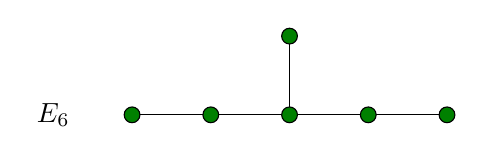
\begin{tikzpicture}

	\draw (0,0) -- (4,0);
	\draw (2,0) -- (2,1);
	
	\draw[fill=Green] (0,0) circle(.1);
	\draw[fill=Green] (1,0) circle(.1);
	\draw[fill=Green] (2,0) circle(.1);
	\draw[fill=Green] (2,1) circle(.1);
	\draw[fill=Green] (3,0) circle(.1);
	\draw[fill=Green] (4,0) circle(.1);
	
	\node at (-1,0) {$E_6$};
	 
\end{tikzpicture}

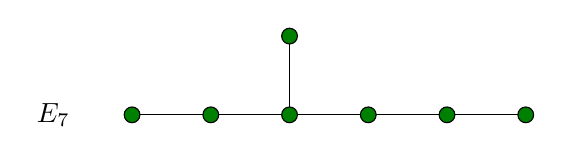
\begin{tikzpicture}

	\draw (0,0) -- (5,0);
	\draw (2,0) -- (2,1);
	
	\draw[fill=Green] (0,0) circle(.1);
	\draw[fill=Green] (1,0) circle(.1);
	\draw[fill=Green] (2,0) circle(.1);
	\draw[fill=Green] (2,1) circle(.1);
	\draw[fill=Green] (3,0) circle(.1);
	\draw[fill=Green] (4,0) circle(.1);
	\draw[fill=Green] (5,0) circle(.1);
	
	\node at (-1,0) {$E_7$};
	 
\end{tikzpicture}

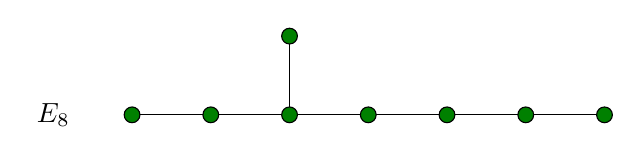
\begin{tikzpicture}

	\draw (0,0) -- (6,0);
	\draw (2,0) -- (2,1);
	
	\draw[fill=Green] (0,0) circle(.1);
	\draw[fill=Green] (1,0) circle(.1);
	\draw[fill=Green] (2,0) circle(.1);
	\draw[fill=Green] (2,1) circle(.1);
	\draw[fill=Green] (3,0) circle(.1);
	\draw[fill=Green] (4,0) circle(.1);
	\draw[fill=Green] (5,0) circle(.1);
	\draw[fill=Green] (6,0) circle(.1);
	
	\node at (-1,0) {$E_8$};
	 
\end{tikzpicture}

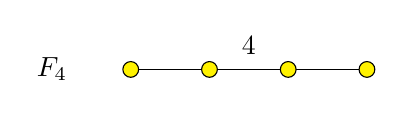
\begin{tikzpicture}

	\draw (0,0) -- (3,0);
	
	\draw[fill=yellow] (0,0) circle(.1);
	\draw[fill=yellow] (1,0) circle(.1);
	\draw[fill=yellow] (2,0) circle(.1);
	\draw[fill=yellow] (3,0) circle(.1);
	
	\node at (1.5, .3) {4};
	\node at (-1,0) {$F_4$};
	 
\end{tikzpicture}

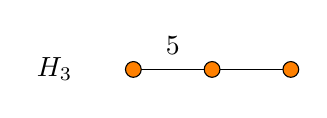
\begin{tikzpicture}

	\draw (0,0) -- (2,0);
	
	\draw[fill=orange] (0,0) circle(.1);
	\draw[fill=orange] (1,0) circle(.1);
	\draw[fill=orange] (2,0) circle(.1);
	
	\node at (.5, .3) {5};
	\node at (-1,0) {$H_3$};
	 
\end{tikzpicture}

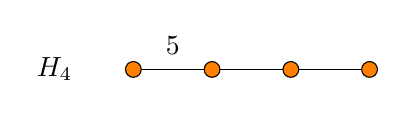
\begin{tikzpicture}

	\draw (0,0) -- (3,0);
	
	\draw[fill=orange] (0,0) circle(.1);
	\draw[fill=orange] (1,0) circle(.1);
	\draw[fill=orange] (2,0) circle(.1);
	\draw[fill=orange] (3,0) circle(.1);
	
	\node at (.5, .3) {5};
	\node at (-1,0) {$H_4$};
	 
\end{tikzpicture}

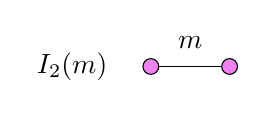
\begin{tikzpicture}

	\draw (0,0) -- (1,0);
	
	\draw[fill=Violet] (0,0) circle(.1);
	\draw[fill=Violet] (1,0) circle(.1);
	
	\node at (.5, .3) {$m$};
	\node at (-1,0) {$I_2(m)$};
	 
\end{tikzpicture}

\end{multicols}

\bigskip

If $\Phi$ is an irreducible root system of rank $\ell$, its Dynkin diagram is one of the following ($\ell$ vertices in each case):

\begin{multicols}{2}

\begin{tikzpicture}
	\fill[color=white] (0,0) circle(.1);
\end{tikzpicture}

\begin{tikzpicture}

	\draw (0,0) -- (1,0);
         \draw (2,0) -- (2.7,0);
         \draw (1,0) -- (2,0);
	\draw (3.3, 0) -- (4,0);
	\draw (4,0) -- (5,0);
	
	\draw[fill=white] (0,0) circle(.1);
	\draw[fill=white] (1,0) circle(.1);
	\draw[fill=white] (2,0) circle(.1);
	\draw[fill=white] (4,0) circle(.1);
	\draw[fill=white] (5,0) circle(.1);
	
	\node at (3,0) {$\cdots$};
	\node at (-1,0) {$A_{\ell}$};
	 
\end{tikzpicture}

\vfill

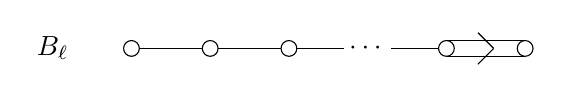
\begin{tikzpicture}

	\draw (0,0) -- (2.7,0);
	\draw (3.3, 0) -- (4,0);
	\draw (4,0.1) -- (5,0.1);
	\draw (4,-0.1) -- (5,-0.1);
	\draw (4.4,0.2) -- (4.6,0);
	\draw (4.4,-0.2) -- (4.6,0);
		
	\draw[fill=white] (0,0) circle(.1);
	\draw[fill=white] (1,0) circle(.1);
	\draw[fill=white] (2,0) circle(.1);
	\draw[fill=white] (4,0) circle(.1);
	\draw[fill=white] (5,0) circle(.1);
	
	\node at (3,0) {$\cdots$};
	\node at (-1,0) {$B_{\ell}$};
	 
\end{tikzpicture}

\vfill

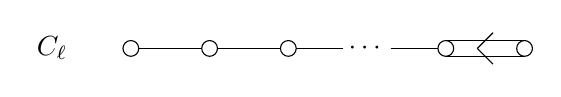
\begin{tikzpicture}

	\draw (0,0) -- (2.7,0);
	\draw (3.3, 0) -- (4,0);
	\draw (4,0.1) -- (5,0.1);
	\draw (4,-0.1) -- (5,-0.1);
	\draw (4.4,0) -- (4.6,0.2);
	\draw (4.4,0) -- (4.6,-0.2);
		
	\draw[fill=white] (0,0) circle(.1);
	\draw[fill=white] (1,0) circle(.1);
	\draw[fill=white] (2,0) circle(.1);
	\draw[fill=white] (4,0) circle(.1);
	\draw[fill=white] (5,0) circle(.1);
	
	\node at (3,0) {$\cdots$};
	\node at (-1,0) {$C_{\ell}$};
	 
\end{tikzpicture}

\vfill

\begin{tikzpicture}

	\draw (0,0) -- (2.7,0);
	\draw (3.3, 0) -- (4,0);
	\draw (4,0) -- (5,-.5);
	\draw (4,0) -- (5,.5);
	
	\draw[fill=white] (0,0) circle(.1);
	\draw[fill=white] (1,0) circle(.1);
	\draw[fill=white] (2,0) circle(.1);
	\draw[fill=white] (4,0) circle(.1);
	\draw[fill=white] (5,-.5) circle(.1);
	\draw[fill=white] (5,.5) circle(.1);
	
	\node at (3,0) {$\cdots$};
	\node at (-1,0) {$D_{\ell}$};
	 
\end{tikzpicture}

\columnbreak

\begin{tikzpicture}

	\draw (0,0) -- (4,0);
	\draw (2,0) -- (2,1);
	
	\draw[fill=white] (0,0) circle(.1);
	\draw[fill=white] (1,0) circle(.1);
	\draw[fill=white] (2,0) circle(.1);
	\draw[fill=white] (2,1) circle(.1);
	\draw[fill=white] (3,0) circle(.1);
	\draw[fill=white] (4,0) circle(.1);
	
	\node at (-1,0) {$E_6$};
	 
\end{tikzpicture}

\vfill

\begin{tikzpicture}

	\draw (0,0) -- (5,0);
	\draw (2,0) -- (2,1);
	
	\draw[fill=white] (0,0) circle(.1);
	\draw[fill=white] (1,0) circle(.1);
	\draw[fill=white] (2,0) circle(.1);
	\draw[fill=white] (2,1) circle(.1);
	\draw[fill=white] (3,0) circle(.1);
	\draw[fill=white] (4,0) circle(.1);
	\draw[fill=white] (5,0) circle(.1);
	
	\node at (-1,0) {$E_7$};
	 
\end{tikzpicture}

\vfill

\begin{tikzpicture}

	\draw (0,0) -- (6,0);
	\draw (2,0) -- (2,1);
	
	\draw[fill=white] (0,0) circle(.1);
	\draw[fill=white] (1,0) circle(.1);
	\draw[fill=white] (2,0) circle(.1);
	\draw[fill=white] (2,1) circle(.1);
	\draw[fill=white] (3,0) circle(.1);
	\draw[fill=white] (4,0) circle(.1);
	\draw[fill=white] (5,0) circle(.1);
	\draw[fill=white] (6,0) circle(.1);
	
	\node at (-1,0) {$E_8$};
	 
\end{tikzpicture}

\vspace{.2in}

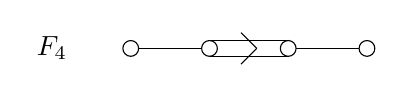
\begin{tikzpicture}

	\draw (0,0) -- (1,0);
	\draw (1,.1) -- (2,.1);
	\draw (1,-.1) -- (2,-.1);
	\draw(2,0) -- (3,0);
	\draw (1.4,0.2) -- (1.6,0);
	\draw (1.4,-0.2) -- (1.6,0);
	
	\draw[fill=white] (0,0) circle(.1);
	\draw[fill=white] (1,0) circle(.1);
	\draw[fill=white] (2,0) circle(.1);
	\draw[fill=white] (3,0) circle(.1);
	
	\node at (-1,0) {$F_4$};
	 
\end{tikzpicture}

\vspace{.2in}

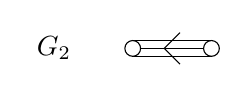
\begin{tikzpicture}

	\draw (0,0) -- (1,0);
	\draw (0,.1) -- (1,.1);
	\draw (0,-.1) -- (1,-.1);
	\draw (.4,0) -- (.6,0.2);
	\draw (.4,0) -- (.6,-0.2);
	
	\draw[fill=white] (0,0) circle(.1);
	\draw[fill=white] (1,0) circle(.1);
	
	\node at (-1,0) {$G_2$};
	 
\end{tikzpicture}

\end{multicols}


\newpage

\section{Tableau(x)}


Here's a standard Young tableau.

\begin{center}
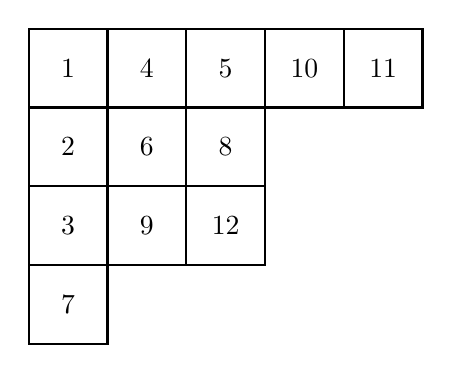
\begin{tikzpicture}[node distance=0 cm,outer sep = 0pt]
	      \node[bsq] (11) at (   1,  1) {1};
	      \node[bsq] (12) [right = of 11] {4};
	      \node[bsq] (13) [right = of 12] {5};
	      \node[bsq] (14) [right = of 13] {10};
	      \node[bsq] (15) [right = of 14] {11};
	      \node[bsq] (21) [below = of 11] {2};
	      \node[bsq] (22) [right = of 21] {6};
	      \node[bsq] (23) [right = of 22] {8};
	      \node[bsq] (31) [below = of 21] {3};
	      \node[bsq] (32) [right = of 31] {9};
	      \node[bsq] (33) [right = of 32] {12};
	      \node[bsq] (41) [below = of 31] {7};
\end{tikzpicture}
\end{center}

Here's a domino tableau.

\begin{center}
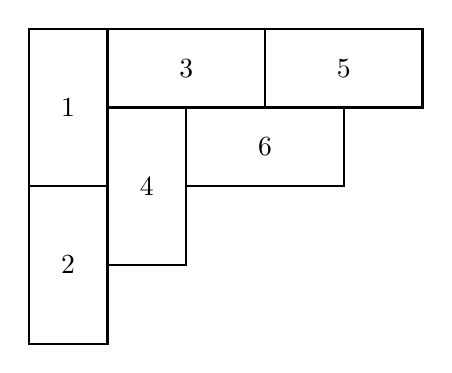
\begin{tikzpicture}[node distance=0 cm,outer sep = 0pt]
        \node[bver] (1) at ( 1.5,   3) {1};
        \node[bver] (2) [below = of 1] {2};
        \node[bhor] (3) at (   3, 3.5) {3};
        \node[bver] (4) at ( 2.5,   2) {4};
        \node[bhor] (5) [right = of 3] {5};
        \node[bhor] (6) at (   4, 2.5) {6};
\end{tikzpicture}  
\end{center}

Both of these images use macros from Tyson Gern -- you'll need to copy these from the header section.

\newpage
\section{Graphs of Functions}

Here's a simple graph of the function $f(x) = x - \frac{x^2}{2} +1$.

\begin{center}
\begin{tikzpicture}
\begin{axis}[ 
	xmin=-2, xmax=2,
	ymin=-3, ymax=3,
	xtick={-2,...,2}, ytick={-3,...,3},
	major tick length={5},
	line width=1pt,
	axis lines=center
	] 
	\addplot [Blue,smooth] {x - 0.5*x^2+1}; 
\end{axis}
\end{tikzpicture}
\end{center}

Here's a graph of a piecewise linear function, with background grid.

\begin{center}
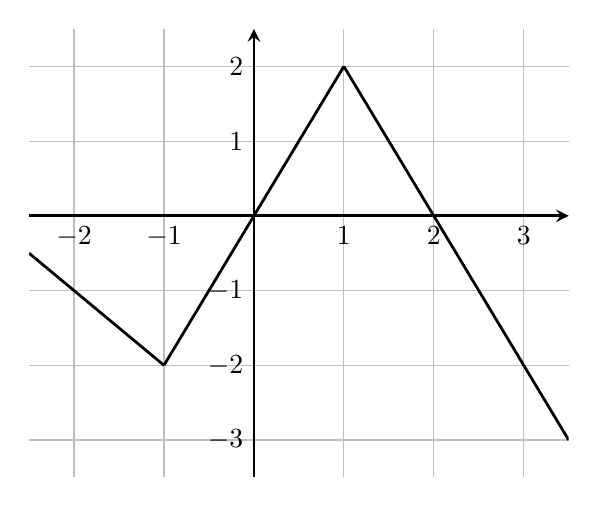
\begin{tikzpicture}
\begin{axis}[ 
	xmin=-2.5, xmax=3.5,
	ymin=-3.5, ymax=2.5,
	xtick={-4,...,4}, ytick={-4,...,4},
	major tick length={0},
	grid=major,
	line width=1pt, % you can take this out, but I find 1pt lines photocopy better than lighter ones
	axis lines=center
	] 
	\addplot [domain=-2.5:-1] {-3-x}; 
	\addplot [domain=-1:1] {2*x}; 
	\addplot [domain=1:3.5] {-2*x+4}; 
\end{axis}
\end{tikzpicture}
\end{center}

\newpage

Here's a graph of $f(x) = \sin(x) - \cos(x)$, with a shaded region.

\begin{center}
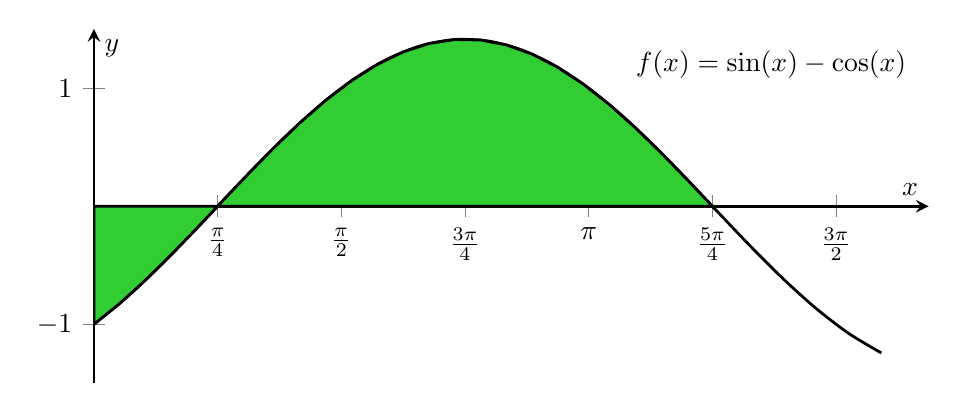
\begin{tikzpicture}
	\begin{axis}[
	y=1.5cm, x=2cm, % this sets the size of one unit along each axis.
	xlabel={$x$}, ylabel={$y$},
	xmin=0, xmax=5.3,
	ymin=-1.5, ymax=1.5,
	xtick={0,0.7853981634,1.570796327,2.35619449,3.141592654,3.926990817,4.71238898}, % tike is dumb with multiples of pi
	ytick={-2,-1,...,2},
	xticklabels={0,$\frac{\pi}{4}$,$\frac{\pi}{2}$,$\frac{3\pi}{4}$,$\pi$,$\frac{5\pi}{4}$,$\frac{3\pi}{2}$}, % so we label them manually
	line width=1pt,
	axis lines=center,
	major tick length={8},
	]
	\addplot [smooth, domain=0:5] {sin(deg(x))-cos(deg(x))}; 
	\addplot [fill=LimeGreen, domain=0:3.926990817] {sin(deg(x))-cos(deg(x))} \closedcycle;
	\node at (axis cs:4.3,1.2) {$f(x) = \sin(x) - \cos(x)$};
\end{axis}
\end{tikzpicture}
\end{center}

Here's another graph, this time with an annoyingly starred region. See p.393 of the \TikZ manual for a list of patterns.

\begin{center}
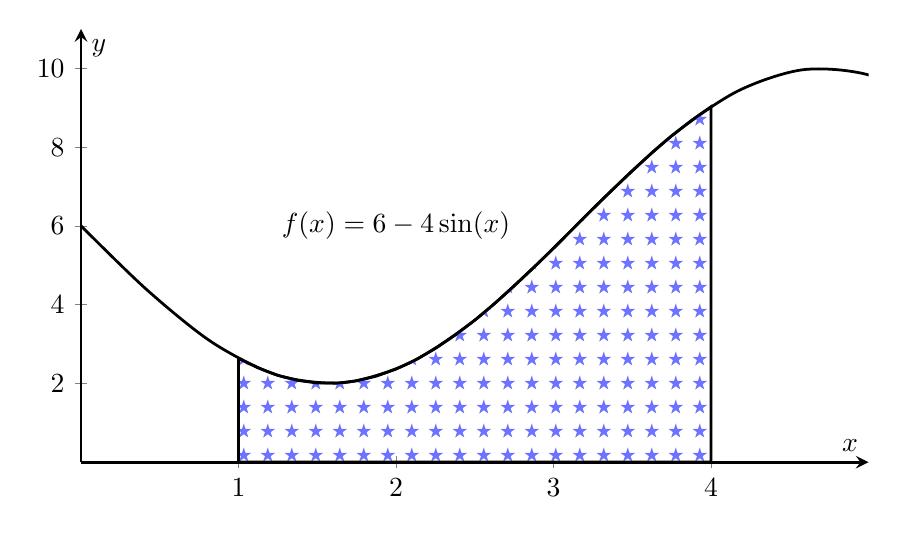
\begin{tikzpicture}[scale=1]
\begin{axis}[
	y=.5cm, x=2cm,
	xlabel={$x$}, ylabel={$y$},
	xmin=0, xmax=5,
	ymin=0, ymax=11,
	xtick={0,1,2,...,4}, ytick={0,2,...,10},
	line width=1pt,
	axis lines=center
	]
	\addplot [smooth, domain=0:10] {-4*sin(deg(x))+6}; 
	\addplot [pattern=fivepointed stars, pattern color=Periwinkle, domain=1:4] {-4*sin(deg(x))+6} \closedcycle;
	\node at (axis cs:2,6) {$f(x) =6-4\sin(x)$};
\end{axis}
\end{tikzpicture}
\end{center}

Here's a function and its tangent line. This graph has a legend.

\begin{center}
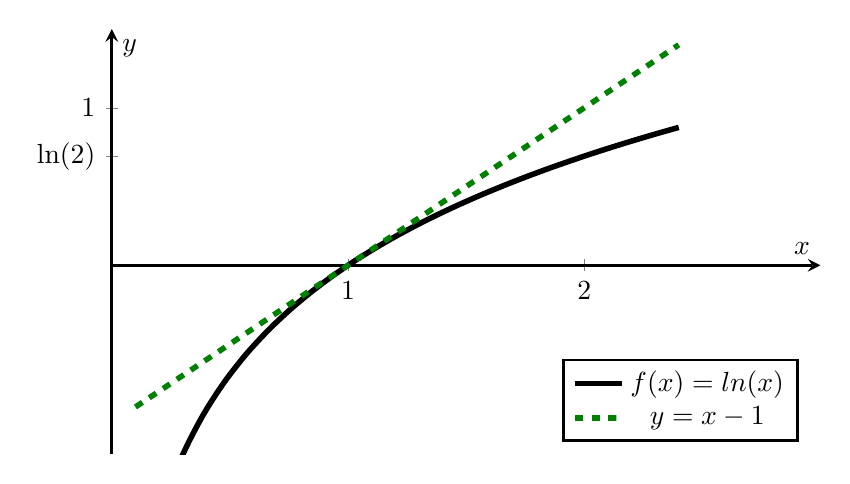
\begin{tikzpicture}
\begin{axis}[
	legend pos=south east,
	y=2cm, x=3cm,
	xlabel={$x$}, ylabel={$y$},
	xmin=0, xmax=3,
	ymin=-1.2, ymax=1.5,
	xtick={0,1,2}, ytick={0,0.6931471806,1},
	xticklabels={0,1,2}, yticklabels={0, $\ln(2)$,1},
	line width=1pt,
	axis lines=center,
	]
	\addplot [smooth, domain=0.2:2.4,line width=2pt] {ln(x)}; 
	\addlegendentry{$f(x) = ln(x)$}
	\addplot [smooth, dashed, line width=2pt,Green, domain=0.1:2.4] {x-1}; 
	\addlegendentry{$y = x - 1$}
\end{axis}
\end{tikzpicture}
\end{center}

\newpage
Here are some various blank axes for a student to draw a graph on.

\begin{center}
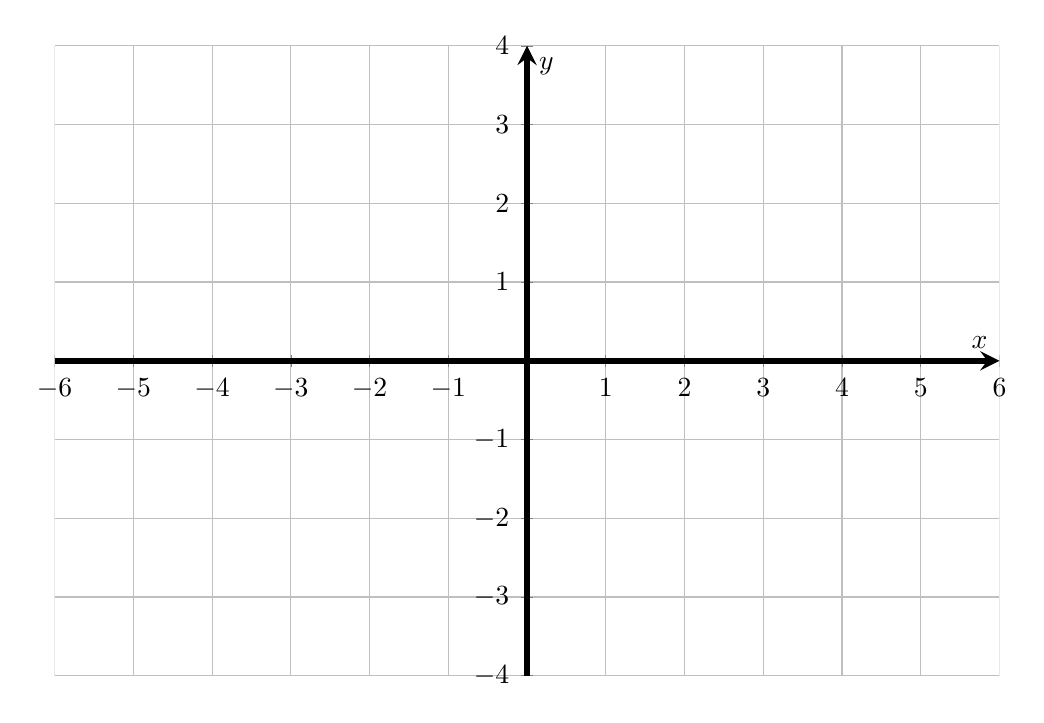
\begin{tikzpicture}
\begin{axis}[ 
	x=1cm, y=1cm,
	xlabel={$x$}, ylabel={$y$},
	xmin=-6, xmax=6,
	ymin=-4, ymax=4,
	xtick={-6,...,6}, ytick={-4,...,4},
	grid=major,
	line width=2pt,
	axis lines=center
	] 
\end{axis}
\end{tikzpicture}
\end{center}

\bigskip

\begin{center}
\begin{tikzpicture}
\begin{axis}[ 
	x=1cm, y=1cm,
	xlabel={$x$}, ylabel={$y$},
	xmin=-6, xmax=6,
	ymin=-4, ymax=4,
	xtick={-5,...,5}, ytick={-3,...,3},
	major tick length={5},
	line width=1pt,
	axis lines=center
	] 
\end{axis}
\end{tikzpicture}
\end{center}

\newpage

Here are some 3d graphs.

\begin{center}
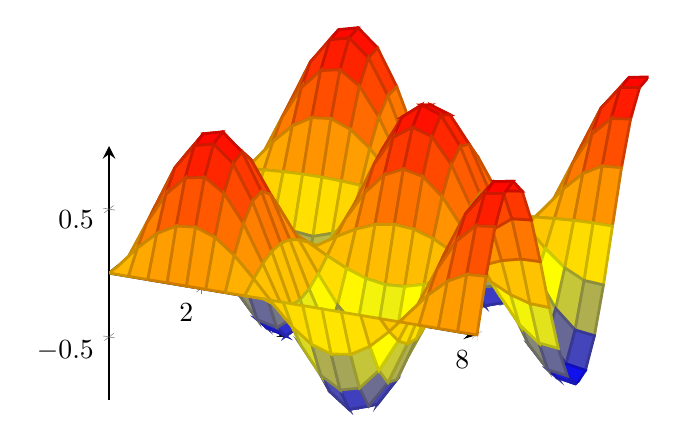
\begin{tikzpicture}
\begin{axis}[axis lines=center,line width=1pt]
\addplot3[surf,domain=0:8,samples=20] {sin(deg(x))*sin(deg(y))};
\end{axis}
\end{tikzpicture}
\end{center}

\bigskip

\begin{center}
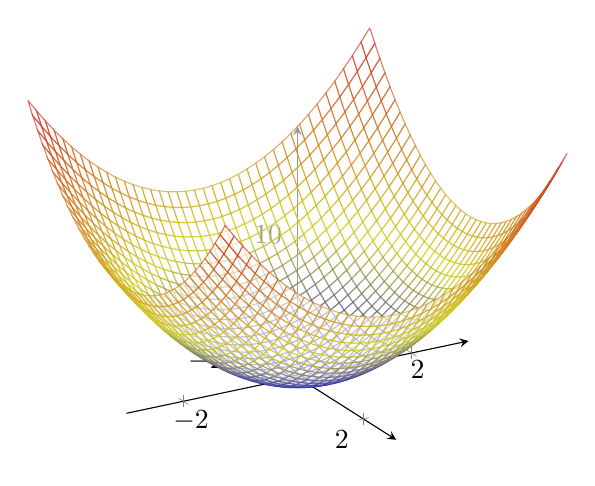
\begin{tikzpicture}
\begin{axis}[view={60}{30},axis lines=center]
\addplot3[surf,fill=white,opacity=0.6,samples=40,
domain=-3:3,y domain=-3:3,
]
{x^2 + y^2};
\end{axis}
\end{tikzpicture}
\end{center}

\newpage
Here is a 3d plot of a parameterized curve:

\begin{center}
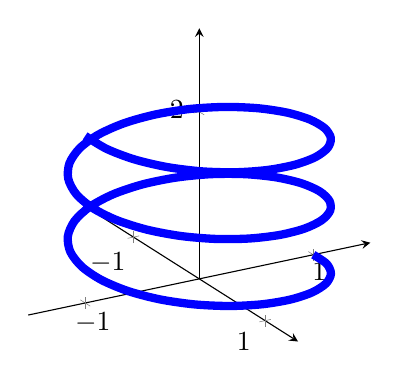
\begin{tikzpicture}
\begin{axis}[view={60}{30},axis lines=center,xmin=-1.5,xmax=1.5,ymin=-1.5,ymax=1.5,zmax=3]
\addplot3+[domain=0:5*pi,samples=60,samples y=0,smooth,mark=none,line width=3pt]
({sin(deg(x))},
{cos(deg(x))},
{2*x/(5*pi)});
\end{axis}
\end{tikzpicture}
\end{center}

\bigskip

And a parameterized torus:

\begin{center}
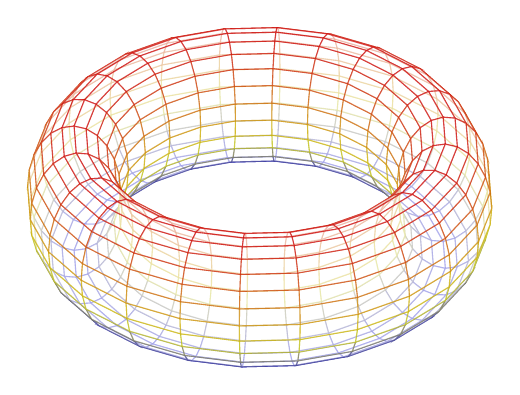
\begin{tikzpicture}
\begin{axis}[view={80}{60},axis lines=none]
\addplot3[surf,fill=white,opacity=0.6,z buffer=sort,domain=0:2*pi,y domain=0:2*pi]
({(4+cos(deg(x))) * cos(deg(y))}, {(4+cos(deg(x))) * sin(deg(y))}, {sin(deg(x))});
\end{axis}
\end{tikzpicture}
\end{center}

\newpage

\section{Vector Diagrams / Root Systems}

Here are some 2d root systems.

\begin{center}
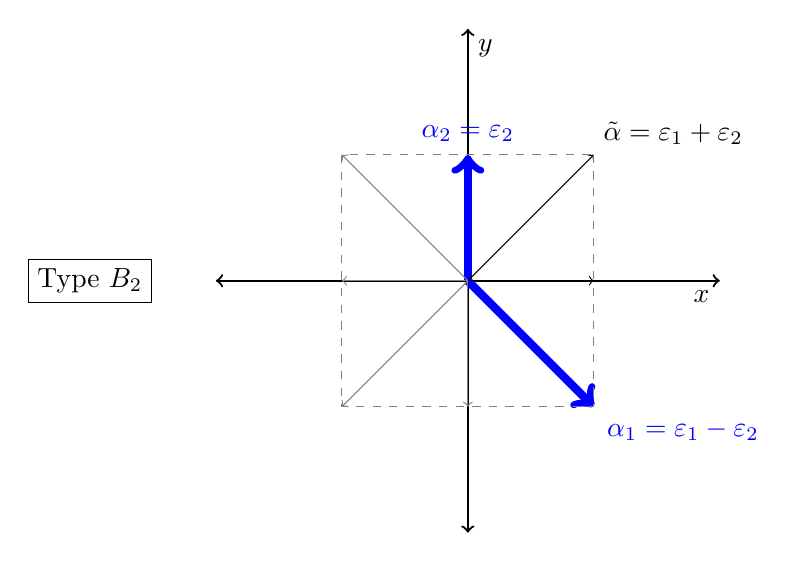
\begin{tikzpicture}[scale=1.6]
	 
	% draw axes
	
	\draw[thick,<->] (-2,0) -- (2,0) node[anchor=north east]{$x$};
	\draw[thick,<->] (0,-2) -- (0,2) node[anchor=north west]{$y$};

	% simple roots

	\draw[line width=3,color=blue,->] (0,0) -- (1,-1) node[anchor=north west]{$\alpha_1 = \varepsilon_1 - \varepsilon_2$};
	\draw[line width=3,color=blue,->] (0,0) -- (0,1) node[anchor=south]{$\alpha_2 = \varepsilon_2$};

	% other positive roots
	
	\draw[->] (0,0) -- (1,1) node[anchor=south west]{$\tilde{\alpha} = \varepsilon_1+\varepsilon_2$};
	\draw[->] (0,0) -- (1,0) ;

	% negative roots
	
	\draw[color=Gray,->] (0,0) -- (-1,1) ;
	\draw[color=Gray,->] (0,0) -- (-1,0) ;
	\draw[color=Gray,->] (0,0) -- (0,-1) ;
	\draw[color=Gray,->] (0,0) -- (-1,-1) ;
	
	% dotted square
	
	\draw[dashed, color=Gray] (1,1) -- (1,-1) -- (-1,-1) -- (-1,1) -- cycle;
	
	\node[rectangle,draw] at (-3,0) {Type $B_2$};
	
\end{tikzpicture}


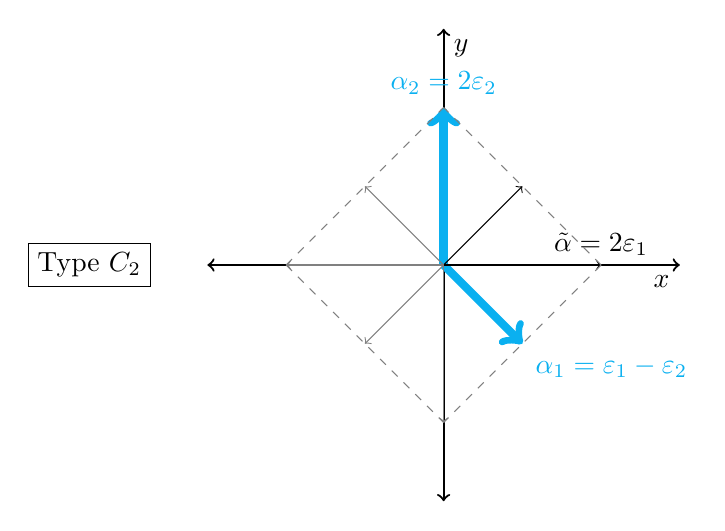
\begin{tikzpicture}
	 
	\draw[thick,<->] (-3,0) -- (3,0) node[anchor=north east]{$x$};
	\draw[thick,<->] (0,-3) -- (0,3) node[anchor=north west]{$y$};

	\draw[line width=3,color=ProcessBlue,->] (0,0) -- (1,-1) node[anchor=north west]{$\alpha_1 = \varepsilon_1 - \varepsilon_2$};
	\draw[line width=3,color=ProcessBlue,->] (0,0) -- (0,2) node[anchor=south]{$\alpha_2 = 2\varepsilon_2$};


	\draw[->] (0,0) -- (1,1) ;
	\draw[color=gray,->] (0,0) -- (-1,1) ;
	\draw[color=gray,->] (0,0) -- (-1,-1) ;

	\draw[color=gray,->] (0,0) -- (-2,0) ;
	\draw[color=gray,->] (0,0) -- (0,-2) ;
	\draw[color=black,->] (0,0) -- (2,0) node[anchor=south]{$\tilde{\alpha} = 2\varepsilon_1$};
	
	\draw[dashed, color=Gray] (2,0) -- (0,2);
	\draw[dashed, color=Gray] (-2,0) -- (0,2);
	\draw[dashed, color=Gray] (-2,0) -- (0,-2);
	\draw[dashed, color=Gray] (2,0) -- (0,-2);
	
	\node[rectangle,draw] at (-4.5,0) {Type $C_2$};

\end{tikzpicture}


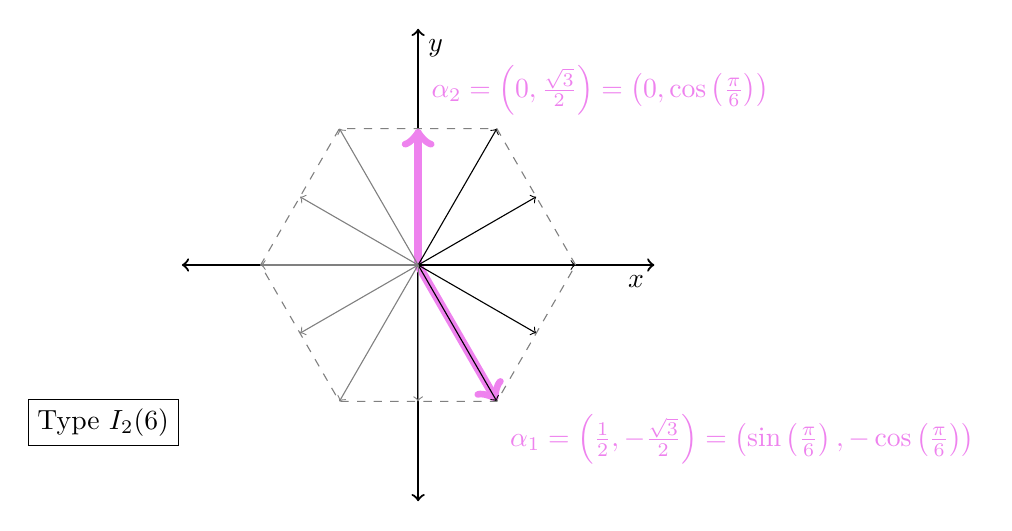
\begin{tikzpicture}[scale=2]
	 
	\draw[thick,<->] (-1.5,0) -- (1.5,0) node[anchor=north east]{$x$};
	\draw[thick,<->] (0,-1.5) -- (0,1.5) node[anchor=north west]{$y$};

	\draw[line width=3,color=Violet,->] (0,0) -- (.5,-.8660254038) node[anchor=north west]{$\alpha_1 = \left(\frac{1}{2}, -\frac{\sqrt{3}}{2}\right) = \left( \sin\left( \frac{\pi}{6} \right), -\cos\left(\frac{\pi}{6}\right) \right)$ };
	\draw[line width=3,color=Violet,->] (0,0) -- (0,.8660254038) node[anchor=south west]{$\alpha_2 = \left( 0,\frac{\sqrt{3}}{2}\right) = \left( 0, \cos\left( \frac{\pi}{6} \right) \right)$};

\draw[->] (0,0) -- (1,0);
\draw[->] (0,0) -- (.5,.8660254038);
\draw[->] (0,0) -- (.5, -.8660254038);

\draw[->] (0,0) -- (.75,.4330127019);
\draw[->] (0,0) -- (.75,-.4330127019);

\draw[color=gray, ->] (0,0) -- (0,-.8660254038);
\draw[color=gray, ->] (0,0) -- (-.5,.8660254038);
\draw[color=gray, ->] (0,0) -- (-.5, -.8660254038);
\draw[color=gray,->] (0,0) -- (-.75,.4330127019);
\draw[color=gray,->] (0,0) -- (-.75,-.4330127019);
\draw[color=gray, ->] (0,0) -- (-1,0);

\draw[dashed, color=gray] (1,0) -- (.5,.8660254038) -- (-.5,.8660254038) -- (-1,0) -- (-.5,-.8660254038) -- (.5,-.8660254038) -- cycle;

	\node[rectangle,draw] at (-2,-1) {Type $I_2(6)$};

\end{tikzpicture}

	
\end{center}


\newpage
Here are some root systems in 3d, using \ttfamily tikz-3dplot\rmfamily.

\begin{center}
\tdplotsetmaincoords{60}{120}
\begin{tikzpicture}[tdplot_main_coords, scale=1.6]

	\coordinate (O) at (0,0,0);
	\tdplotsetcoord{P}{1}{-100}{200}

	\draw[dashed, color=gray] (0,1,-1) -- (1,0,-1) -- (1,-1,0) -- (0,-1,1) -- (-1,0,1) -- (-1,1,0) -- cycle;

	\draw[thick,->] (0,0,0) -- (4,0,0) node[anchor=north east]{$x$};
	\draw[thick,->] (0,0,0) -- (0,2.5,0) node[anchor=north west]{$y$};
	\draw[thick,->] (0,0,0) -- (0,0,2) node[anchor=south]{$z$};

	\draw[line width=3,color=red,->] (0,0,0) -- (1,-1,0) node[anchor=east]{$\alpha_1 = \varepsilon_1 - \varepsilon_2$};
	\draw[line width=3,color=red,->] (0,0,0) -- (0,1,-1) node[anchor=north west]{$\alpha_2 = \varepsilon_2 - \varepsilon_3$};

	\draw[->] (0,0,0) -- (1,0,-1) node[anchor=north]{$\tilde{\alpha} = \varepsilon_1 - \varepsilon_3$};

	\draw[color=gray, ->] (0,0,0) -- (-1,1,0);
	\draw[color=gray, ->] (0,0,0) -- (0,-1,1);
	\draw[color=gray, ->] (0,0,0) -- (-1,0,1);

	\draw[dashed,line width=1, <->] (-.7,-.7,1.4) -- (.7,.7,-1.4) node[anchor=north west]{$s_{\varepsilon_1 - \varepsilon_2}$};
	
	\node[rectangle,draw] at (0,3,2) {Type $A_2$};

\end{tikzpicture}

\bigskip

\tdplotsetmaincoords{80}{110} % change these parameters to rotate the 3d coordinate system
\begin{tikzpicture}[tdplot_main_coords, scale=2]
		 
	\coordinate (O) at (0,0,0);
	\tdplotsetcoord{P}{1}{-100}{200}
	
	% draw axes
	
	\draw[thick,->] (0,0,0) -- (5,0,0) node[anchor=north east]{$x$};
	\draw[thick,->] (0,0,0) -- (0,2.5,0) node[anchor=north west]{$y$};
	\draw[thick,->] (0,0,0) -- (0,0,2) node[anchor=south]{$z$};
	
	% simple roots
	
	\draw[line width=3,color=Magenta,->] (0,0,0) -- (1,-1,0) node[anchor=east]{$\alpha_1 = \varepsilon_1 - \varepsilon_2$};
	\draw[line width=3,color=Magenta,->] (0,0,0) -- (0,1,-1) node[anchor=north west]{$\alpha_2 = \varepsilon_2 - \varepsilon_3$};
	\draw[line width=3,color=Magenta,->] (0,0,0) -- (0,1,1) node[anchor=south west]{$\alpha_3 = \varepsilon_2 + \varepsilon_3$};
	
	% other positive roots
	
	\draw[->] (0,0,0) -- (1,1,0) node[anchor=west]{$\tilde{\alpha} = \varepsilon_1 + \varepsilon_2$};
	\draw[->] (0,0,0) -- (1,0,1) ;
	\draw[->] (0,0,0) -- (1,0,-1);
	
	% negative roots
	
	\draw[color=Gray,->] (0,0,0) -- (-1,0,1) ;
	\draw[color=Gray,->] (0,0,0) -- (-1,1,0) ;
	\draw[color=Gray,->] (0,0,0) -- (0,-1,1) ;
	\draw[color=Gray,->] (0,0,0) -- (-1,0,-1) ;
	\draw[color=Gray,->] (0,0,0) -- (-1,-1,0) ;
	\draw[color=Gray,->] (0,0,0) -- (0,-1,-1) ;
	
	% cube of side length 2
	
	\draw[dashed, color=gray] (1,1,1) -- (1,1,-1);
	\draw[dashed, color=gray] (1,1,1) -- (1,-1,1);
	\draw[dashed, color=gray] (1,1,1) -- (-1,1,1);
	
	\draw[dashed, color=gray] (1,1,-1) -- (-1,1,-1);
	\draw[dashed, color=gray] (1,1,-1) -- (1,-1,-1);
	
	\draw[dashed, color=gray] (1,-1,1) -- (-1,-1,1);
	\draw[dashed, color=gray] (1,-1,1) -- (1,-1,-1);
	
	\draw[dashed, color=gray] (-1,1,1) -- (-1,-1,1);
	\draw[dashed, color=gray] (-1,1,1) -- (-1,1,-1);
	
	\draw[dashed, color=gray] (-1,1,-1) -- (-1,-1,-1);
	\draw[dashed, color=gray] (1,-1,-1) -- (-1,-1,-1);
	\draw[dashed, color=gray] (-1,-1,1) -- (-1,-1,-1);

	\node[rectangle,draw] at (0,-2.5,1) {Type $D_3$};

\end{tikzpicture}
\end{center}


\newpage 


\begin{center}
\tdplotsetmaincoords{80}{110}
\begin{tikzpicture}[tdplot_main_coords, scale=2.6]
	 
	\coordinate (O) at (0,0,0);
	\tdplotsetcoord{P}{1}{-100}{200}
	
	\draw[thick,->] (0,0,0) -- (5,0,0) node[anchor=north east]{$x$};
	\draw[thick,->] (0,0,0) -- (0,2.5,0) node[anchor=north west]{$y$};
	\draw[thick,->] (0,0,0) -- (0,0,2) node[anchor=south]{$z$};
	
	\draw[line width=3,color=blue,->] (0,0,0) -- (1,-1,0) node[anchor=east]{$\alpha_1 = \varepsilon_1 - \varepsilon_2$};
	\draw[line width=3,color=blue,->] (0,0,0) -- (0,1,-1) node[anchor=north west]{$\alpha_2 = \varepsilon_2 - \varepsilon_3$};
	\draw[line width=3,color=blue,->] (0,0,0) -- (0,0,1) node[anchor=south]{$\alpha_3 = \varepsilon_3$};
	
	\draw[->] (0,0,0) -- (1,1,0) node[anchor=west]{$\tilde{\alpha} = \varepsilon_1 + \varepsilon_2$};
	
	\draw[->] (0,0,0) -- (1,0,-1);
	\draw[->] (0,0,0) -- (-1,1,0) ;
	\draw[->] (0,0,0) -- (0,-1,1) ;
	\draw[->] (0,0,0) -- (-1,0,1) ;
	\draw[->] (0,0,0) -- (1,0,1) ;
	\draw[->] (0,0,0) -- (1,1,0) ;
	\draw[->] (0,0,0) -- (0,1,1) ;
	\draw[->] (0,0,0) -- (-1,0,-1) ;
	\draw[->] (0,0,0) -- (-1,-1,0) ;
	\draw[->] (0,0,0) -- (0,-1,-1) ;
	
	\draw[line width=2,color=gray,->] (0,0,0) -- (-1,0,0) ;
	\draw[line width=2,color=gray,->] (0,0,0) -- (0,-1,0) ;
	\draw[line width=2,color=gray,->] (0,0,0) -- (0,0,-1) ;
	\draw[line width=2,color=black,->] (0,0,0) -- (1,0,0) ;
	\draw[line width=2,color=black,->] (0,0,0) -- (0,1,0) ;
	
	
	% CUBE OF SIDE LENGTH 2
	
	\draw[dashed, color=gray] (1,1,1) -- (1,1,-1);
	\draw[dashed, color=gray] (1,1,1) -- (1,-1,1);
	\draw[dashed, color=gray] (1,1,1) -- (-1,1,1);
	
	\draw[dashed, color=gray] (1,1,-1) -- (-1,1,-1);
	\draw[dashed, color=gray] (1,1,-1) -- (1,-1,-1);
	
	\draw[dashed, color=gray] (1,-1,1) -- (-1,-1,1);
	\draw[dashed, color=gray] (1,-1,1) -- (1,-1,-1);
	
	\draw[dashed, color=gray] (-1,1,1) -- (-1,-1,1);
	\draw[dashed, color=gray] (-1,1,1) -- (-1,1,-1);
	
	\draw[dashed, color=gray] (-1,1,-1) -- (-1,-1,-1);
	\draw[dashed, color=gray] (1,-1,-1) -- (-1,-1,-1);
	\draw[dashed, color=gray] (-1,-1,1) -- (-1,-1,-1);
	
	% TETRAHEDRON
	
	\draw[color=gray] (1,0,0) -- (0,1,0) -- (0,0,1) -- cycle;
	\draw[color=gray] (1,0,0) -- (0,-1,0) -- (0,0,1) --  cycle;
	\draw[color=gray] (1,0,0) -- (0,0,-1) -- (0,-1,0) -- cycle;
	\draw[color=gray] (1,0,0) -- (0,0,-1) -- (0,1,0) -- cycle;
	
	\draw[color=gray] (-1,0,0) -- (0,1,0) -- (0,0,1) -- cycle;
	\draw[color=gray] (-1,0,0) -- (0,-1,0) -- (0,0,1) --  cycle;
	\draw[color=gray] (-1,0,0) -- (0,0,-1) -- (0,-1,0) -- cycle;
	\draw[color=gray] (-1,0,0) -- (0,0,-1) -- (0,1,0) -- cycle;

	\node[rectangle,draw] at (0,2,2) {Type $B_3$};

\end{tikzpicture}

\bigskip

\tdplotsetmaincoords{80}{110}
\begin{tikzpicture}[tdplot_main_coords, scale=2]
	 
	\coordinate (O) at (0,0,0);
	\tdplotsetcoord{P}{1}{-100}{200}
	
	\draw[thick,->] (0,0,0) -- (6,0,0) node[anchor=north east]{$x$};
	\draw[thick,->] (0,0,0) -- (0,3.5,0) node[anchor=north west]{$y$};
	\draw[thick,->] (0,0,0) -- (0,0,3) node[anchor=south]{$z$};
	
	\draw[line width=3,color=ProcessBlue,->] (0,0,0) -- (1,-1,0) node[anchor=east]{$\alpha_1 = \varepsilon_1 - \varepsilon_2$};
	\draw[line width=3,color=ProcessBlue,->] (0,0,0) -- (0,1,-1) node[anchor=north west]{$\alpha_2 = \varepsilon_2 - \varepsilon_3$};
	\draw[line width=3,color=ProcessBlue,->] (0,0,0) -- (0,0,2) node[anchor=south]{$\alpha_3 = 2\varepsilon_3$};
	
	\draw[->] (0,0,0) -- (1,1,0);
	\draw[->] (0,0,0) -- (1,0,-1);
	\draw[->] (0,0,0) -- (-1,1,0) ;
	\draw[->] (0,0,0) -- (0,-1,1) ;
	\draw[->] (0,0,0) -- (-1,0,1) ;
	\draw[->] (0,0,0) -- (1,0,1) ;
	\draw[->] (0,0,0) -- (1,1,0) ;
	\draw[->] (0,0,0) -- (0,1,1) ;
	\draw[->] (0,0,0) -- (-1,0,-1) ;
	\draw[->] (0,0,0) -- (-1,-1,0) ;
	\draw[->] (0,0,0) -- (0,-1,-1) ;
	
	\draw[line width=2,color=Gray,->] (0,0,0) -- (-2,0,0) ;
	\draw[line width=2,color=Gray,->] (0,0,0) -- (0,-2,0) ;
	\draw[line width=2,color=Gray,->] (0,0,0) -- (0,0,-2) ;
	\draw[line width=2,->] (0,0,0) -- (2,0,0) node[anchor=north east]{$\tilde{\alpha} = 2\varepsilon_1$} ;
	\draw[line width=2,color=black,->] (0,0,0) -- (0,2,0)  ;
	
	% CUBE OF SIDE LENGTH 2
	
	\draw[dashed, color=gray] (1,1,1) -- (1,1,-1);
	\draw[dashed, color=gray] (1,1,1) -- (1,-1,1);
	\draw[dashed, color=gray] (1,1,1) -- (-1,1,1);
	
	\draw[dashed, color=gray] (1,1,-1) -- (-1,1,-1);
	\draw[dashed, color=gray] (1,1,-1) -- (1,-1,-1);
	
	\draw[dashed, color=gray] (1,-1,1) -- (-1,-1,1);
	\draw[dashed, color=gray] (1,-1,1) -- (1,-1,-1);
	
	\draw[dashed, color=gray] (-1,1,1) -- (-1,-1,1);
	\draw[dashed, color=gray] (-1,1,1) -- (-1,1,-1);
	
	\draw[dashed, color=gray] (-1,1,-1) -- (-1,-1,-1);
	\draw[dashed, color=gray] (1,-1,-1) -- (-1,-1,-1);
	\draw[dashed, color=gray] (-1,-1,1) -- (-1,-1,-1);
	
	% TETRAHEDRON
	
	\draw[color=gray] (2,0,0) -- (0,2,0) -- (0,0,2) -- cycle;
	\draw[color=gray] (2,0,0) -- (0,-2,0) -- (0,0,2) -- cycle;
	\draw[color=gray] (2,0,0) -- (0,0,-2) -- (0,-2,0) -- cycle;
	\draw[color=gray] (2,0,0) -- (0,0,-2) -- (0,2,0) -- cycle;
	
	\draw[color=gray] (-2,0,0) -- (0,2,0) -- (0,0,2) -- cycle;
	\draw[color=gray] (-2,0,0) -- (0,-2,0) -- (0,0,2) -- cycle;
	\draw[color=gray] (-2,0,0) -- (0,0,-2) -- (0,-2,0) -- cycle;
	\draw[color=gray] (-2,0,0) -- (0,0,-2) -- (0,2,0) -- cycle;

	\node[rectangle,draw] at (0,2,2) {Type $C_3$};

\end{tikzpicture}



\end{center}




\newpage

\section{Adding extra space in tables}

Here's a table with a little extra height added to the columns and extra padding added in the cells:

\begin{center}
{ \renewcommand{\arraystretch}{1.8} % stretches the row height
\setlength{\tabcolsep}{10pt} % adds horizontal padding
\begin{tabular}{|c|c|c|c|c|c|} \hline
$x$ &0&${\pi/4} $&${\pi/2} $ &${3\pi/4} $ &${\pi} $ \\ \hline 
$\cos(x)$ &1 &$\sqrt2/2$ &0 &$-\sqrt{2}/{2}$ &$-1$ \\ \hline 
$\sin(x)$ &0 &$\sqrt2/2$ &1 &$\sqrt{2}/{2}$ &$0$ \\ \hline 
\end {tabular}
}
\end{center}  


\vfill\eject
\end{document}
